\documentclass[10pt,a4paper]{article}
\usepackage[utf8]{inputenc}
\usepackage{amsmath}
\usepackage{amsfonts}
\usepackage{amssymb}
\usepackage[left=2cm,right=2cm,top=2cm,bottom=2cm]{geometry}
\usepackage{url}
\usepackage{graphicx}
\usepackage[per-mode=symbol]{siunitx}
% Package for hyperlink, without ugly box around and nice blue color for text
\usepackage{hyperref}
\usepackage{xcolor}
\hypersetup{
	colorlinks,
	linkcolor={red!50!black},
	citecolor={blue!50!black},
	urlcolor={blue!80!black}
}

\usepackage[
    type={CC},
    modifier={by-sa},
    version={4.0},
]{doclicense}

\begin{document}
\title{Exercise 4: IDEAS Tutorial - part 2}
\author{Filip Jorissen, Damien Picard\\ \thanks{Review} Jelger Jansen, Iago Cupeiro Figueroa, Lucas Verleyen}
\date{KU Leuven, September 23, 2022}
\maketitle

\doclicenseThis

\section*{Introduction}
The goal of this exercise is to become familiar with the 
Modelica packages of IDEAS that are
complementary to \path{IDEAS.Buildings} used in Exercise 3. \\

For this exercise you will extend the model of a simple house,
using HVAC and other components.
This exercise starts/extends from the model \path{IDEAS.Examples.Tutorial.Example5}. 
Model complexity will be increased in each step by 
extending the model from the previous step, i.e. for each step a new model should be created that uses
the Modelica \path{extends} clause to extend the previous model.
In between steps, the result differences can be compared.\\


In the following sections the exercise is discussed 
in several steps. 
Each step first qualitatively explains the model part.
Secondly, the names of the required IDEAS models 
are listed.
Thirdly, we provide high-level instructions of how to
set up the model.
If these instructions are not clear immediately, 
have a look at the model documentation and at the type of
connectors the model has, 
try out some things, 
make an educated guess, etc.
Depending on the parameter values that you choose, results
may differ slightly.
We also list some side notes, which are not strictly required for this
exercise, but which may help you to effectively use Modelica
and IDEAS in the future.
In some cases we list some important background information.\\

The main packages that you will need, are:
\begin{enumerate}
\item \path{IDEAS.Fluid}: a package containing air flow and hydronic system components.
\item \path{IDEAS.Media}: a package containing commonly used media implementations that are tailored to building applications.
\item \path{IDEAS.Utilities}: a package containing components that simplify model development and automation of workflows.
\end{enumerate}

\section{Heating system}
\paragraph{Qualitative discussion}
In this step you will extend the model \path{IDEAS.Examples.Tutorial.Example5} 
by adding a HVAC system.
The system consists of a water-water heat pump, radiators, 
a storage tank,
circulation pumps and a low temperature heat source for the heat pump.
Use constant control set points for the heat pump and pumps.
Add a system that measures the heat pump electrical energy use.\\
\newpage

\paragraph{Required models}
This step requires the following components:
\begin{itemize}
\item \path{IDEAS.Fluid.HeatPumps.ScrollWaterToWater}
\item \path{IDEAS.Fluid.HeatExchangers.Radiators.RadiatorEN442_2}
\item \path{IDEAS.Fluid.Actuators.Valves.TwoWayTRV}
\item \path{IDEAS.Fluid.Movers.FlowControlled_dp}
\item \path{IDEAS.Fluid.Sources.Boundary_pT}
\item \path{IDEAS.Media.Water}
\item \path{IDEAS.Fluid.Storage.Stratified}
\item \path{Modelica.Blocks.Sources.IntegerConstant}
\item \path{Modelica.Blocks.Continuous.Integrator}
\end{itemize}

\paragraph{Important notes on Fluid system modelling}
The model components of \path{IDEAS.Buildings} have been integrated where possible.
E.g. a zone can always have an occupancy schedule, or lighting models. 
However, for HVAC, many configurations exist in reality. 
Some zones have a radiator, which physically resides within the zone, 
while others may use floor heating, which is a property of the floor.
Some zones may even have multiple radiators with different sizes, etc.
Due to this multitude of options, HVAC components have not been integrated into
the \path{IDEAS.Buildings} components (yet).
Instead, they can be added manually by the user.
This requires some knowledge by the user about how to interconnect the different components, 
and even about the relevant physical principles that are at play. \\

One notable example is the fact that we use pressure-driven flow models 
to compute mass flow rates through hydronic systems, i.e. the mass flow rates are computed from pressure drop equations
and the pump head that is generated by a pump.
The advantage is that 
pump and fan powers can be computed accurately and 
complex hydronic systems can be modelled, 
where Modelica will automatically deduce the mass flow rate in each branch.
The disadvantage is that (somewhat) realistic pressure drop parameters have to be supplied
to the model.
An alternative modelling approach, which is commonly used by other building energy simulation tools, 
is to `outsmart' physics and to directly prescribe mass flow rates.
Depending on the user experience, it is however easy to make modelling errors that cause
non-physical results or non-physical models, which cause Dymola to throw a `singular system' error.
For instance, when prescribing a flow (instead of pressure),
the situation can occur where a flow rate is forced
through a closed valve, which is not possible in practice. 
Our model equations will predict a huge
pressure drop over the valve, which can easily lead to a pump power 
of a few MW and a large
temperature increase of the water when passing though the pump\footnote{Since the model assumes that the flow work 
is injected into the stream as a thermal power.}.\\

To summarize, modelling fluid flows in Modelica can be quite involved,
but you can achieve a high level of detail in doing so.
Proceed with care, think about how a system physically works and make sure to 
include all relevant components.
One notable example is that in each fluid loop the 
\textit{absolute} pressure of that loop has to be defined somewhere: 
pumps and valves only provide information
about \textit{differential} pressures. 
For this purpose use \path{IDEAS.Fluid.Sources.Boundary_pT} and connect
it to the loop, which will set the absolute pressure at the connection point.


\paragraph{Instructions}
Start by adding one radiator for each zone and by 
connecting them to the respective zone models using the (red) heat ports.
See the port documentation\footnote{By hovering your mouse over the port.} 
for more hints about how to do so.
The radiator parameters can be set to 500~$W$, 45$^{\circ}C$/35$^{\circ}C$ inlet/outlet\footnote{From these \textit{nominal} values, the model computes the \textit{actual} heat flow rate based on the \textit{actual} inlet temperature.}
and a pressure drop of 0~$Pa$\footnote{We here implicitly assume that the radiator pressure drop is negligible compared to the valve pressure drop, which we are about to add.}.\\

Typically, radiators have a Thermostatic Radiator Valve (TRV)
that automatically reduces the flow towards the radiator
when the zone temperature is sufficiently high.
We model this by adding a TRV model, which uses
the zone temperature \path{TSensor} as an input.
Physically, each radiator has its own TRV, 
so this should be reflected in the model.
The nominal mass flow rate of the valve can be set to the nominal
mass flow rate of the respective radiator and its nominal pressure drop can be set 
to 20~$kPa$.\\

Add a heat pump. 
Use performance data for the \textit{Viessmann Vitocal 300G BW 301.A21} heat pump.
These performance data are for a 21~$kW$ heat pump, 
which is much more than we require for our heating system (2 radiators of 500~$W$).
Therefore set the heat pump scaling factor to 0.025, 
which rescales the heat pump behaviour to a thermal power of 525~$W$.
Furthermore, choose realistic nominal mass flow rates and set the nominal pressure
drop to 10~$kPa$. Set \path{enable_variable_speed=false} and set the control input (orange triangle)
such that the heat pump is on using an \path{IntegerConstant}.\\

Add a storage tank that buffers the warm water that is produced.
Connect the storage tank at the secondary (the warm side) outlet of the heat pump.
Choose a volume of 100~$l$ (0.1~$m^3$), a height of 0.5~$m$ and an insulation thickness of 10~$cm$.\\

Add two pumps.
At the secondary side of the heat pump, 
set the pump nominal flow rate to the sum of the radiator nominal flow rates
and set the nominal pressure head to 20~$kPa$.
At the primary side, do the same.
Both pumps should always be on.\\

The primary side of the heat pump and its circulation pump should be connected
to a heat source. Use the model \path{IDEAS.Fluid.Sources.Boundary_pT} for this,
which acts as a fluid source and a fluid sink. You can specify the pressure
and the temperature of the fluid. Set the temperature to 10$^{\circ}C$.\\

Add \textit{water} as a \path{Medium} to the model 
in the text view (\path{IDEAS.Media.Water}), and use it in all components. Compute the electrical energy by integrating the electrical power of the heat pump
using an \path{Integrator}. A reference implementation for this example is shown in Figure~\ref{fig:sche}.



\paragraph{Side notes}
By default, the Dymola `canvas' has a size of 100 pt by 100 pt. 
When extending a model  it can sometimes be useful to enlarge this canvas size by dragging
the corners of the (white) canvas. 
This avoids a lot of scrolling across the model.\\

IDEAS has multiple heat pump models, which have a different level of detail
and which use a different set of parameters as an input.
The models \path{IDEAS.Fluid.HeatPumps.ScrollWaterToWater}
and \path{IDEAS.Fluid.HeatPumps.ReciprocatingWaterToWater} are
the most physically detailed models and should be used whenever possible.\\

Modelica uses SI units by default, which means that temperatures by default 
are presented with the units of Kelvin. However, if you plot results in Dymola, you can often change $K$ to $^{\circ}C$ in the plot interface. \\



\begin{figure}[h]
\centering
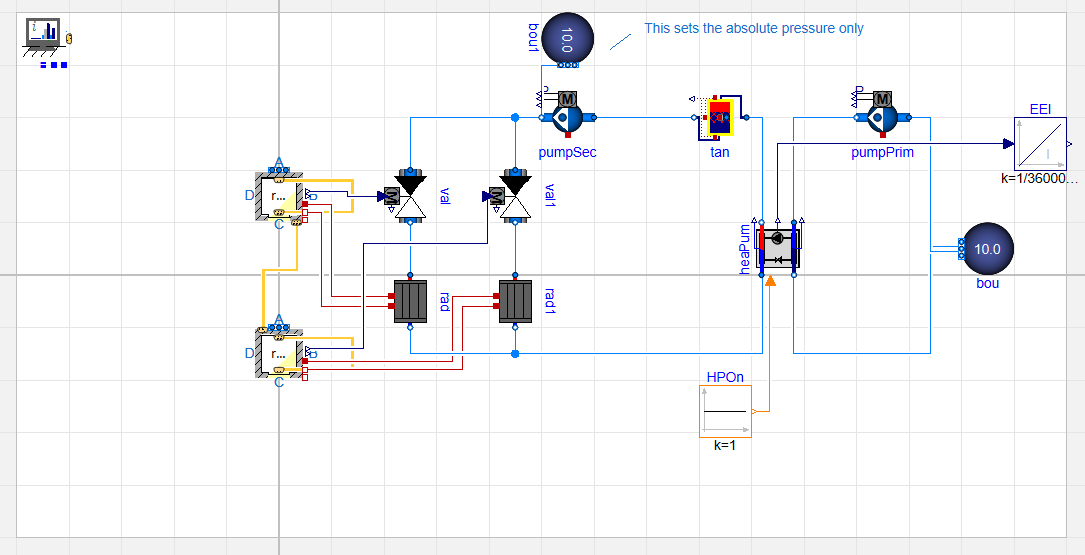
\includegraphics[width=\linewidth]{Schematic6.png}
\caption{The schematic of Example 6.}
\label{fig:sche}
\end{figure}

\paragraph{Reference result}
We simulate this model with the settings
\begin{enumerate}
\item Start time = 1e7,
\item Stop time = 1.1e7,
\item Number of intervals = 5000.
\end{enumerate}
We thus perform a simulation that starts $10^7$ seconds after new year and ends $10^6$
seconds later, which is a period of 11.6 days. Remark that the simulation time of this model will be significantly higher ($\sim$1 minute) than those of the models previoulsy developed in this crash course. The explanation follows below. You can track the simulation progress at the bottom of the Dymola window. \\


We now plot the zone temperatures \path{rectangularZoneTemplate.TSensor} and \path{rectangularZoneTemplate1.TSensor}, the radiator heat flow rates \path{rad.Q_flow} and \path{rad1.Q_flow}, the heat pump condenser temperature \path{heaPum.con.T} and the heat pump heat flow rate \path{heaPum.QCon_flow}. The results are shown in Figure~\ref{fig:res1} and Figure~\ref{fig:res1_bis} and deserve some explanation.\\

Firstly, we see that the zone temperatures are quite different. This is because the orientation of the windows. In the northern zone (\path{rectangularZoneTemplate}), there is only one window oriented towards the north, whereas in the southern zone (\path{rectangularZoneTemplate1}), there is only one window oriented towards the south. Much more solar irradiation will reach the southern zone by its window and leads to an increased zone temperature. As there is only solar irradiation during the day, you clearly see the day/night fluctuations. When the zone temperatures drop below the 21$^{\circ}C$ set point temperature (mostly during the night), the TRVs will open and a higher mass flow rate will flow through the radiators wich leads to a higher thermal power emitted by the radiators.\\

When the TRVs are closed, the heat pump is still switched on (because we applied a constant integer input equal to 1). Consequently, the supply water temperature of the radiators rises up to 65$^{\circ}C$, even though the radiator nominal dimensions are for a supply water temperature of
45$^{\circ}C$. The elevated temperatures mean that the radiators can
emit a higher than nominal thermal power.
However, in the bottom graph the radiator thermal power never surpasses
even half of its nominal value.
This is caused by the thermostatic valves, which reduce the mass flow rate
that enters the radiator, and consequently lowers the thermal power. \\

This reduced mass flow rate when there is no heat demand in the zone and a heat pump which is always switched on due to the applied input signal, causes a high temperature at the condenser side of the heat pump and a large temperature difference across the heat pump (primary heat source of 10$^{\circ}C$),
The heat pump model contains a built-in temperature protection, which disables
the heat pump when the temperature exceeds a predefined threshold.
Consequently, the heat pump continuously switches on and off
and operates at high temperatures for most of the time.
This switching also negatively impacts the computation time, 
as you may have noticed.\\

This example illustrates the importance of control, which is currently not modelled.
All pumps and the heat pump are assumed to be active continuously, 
which is detrimental for the system performance.
The COP (\path{heaPum.com.COP}) is only about 2.9.


\begin{figure}[h]
\centering
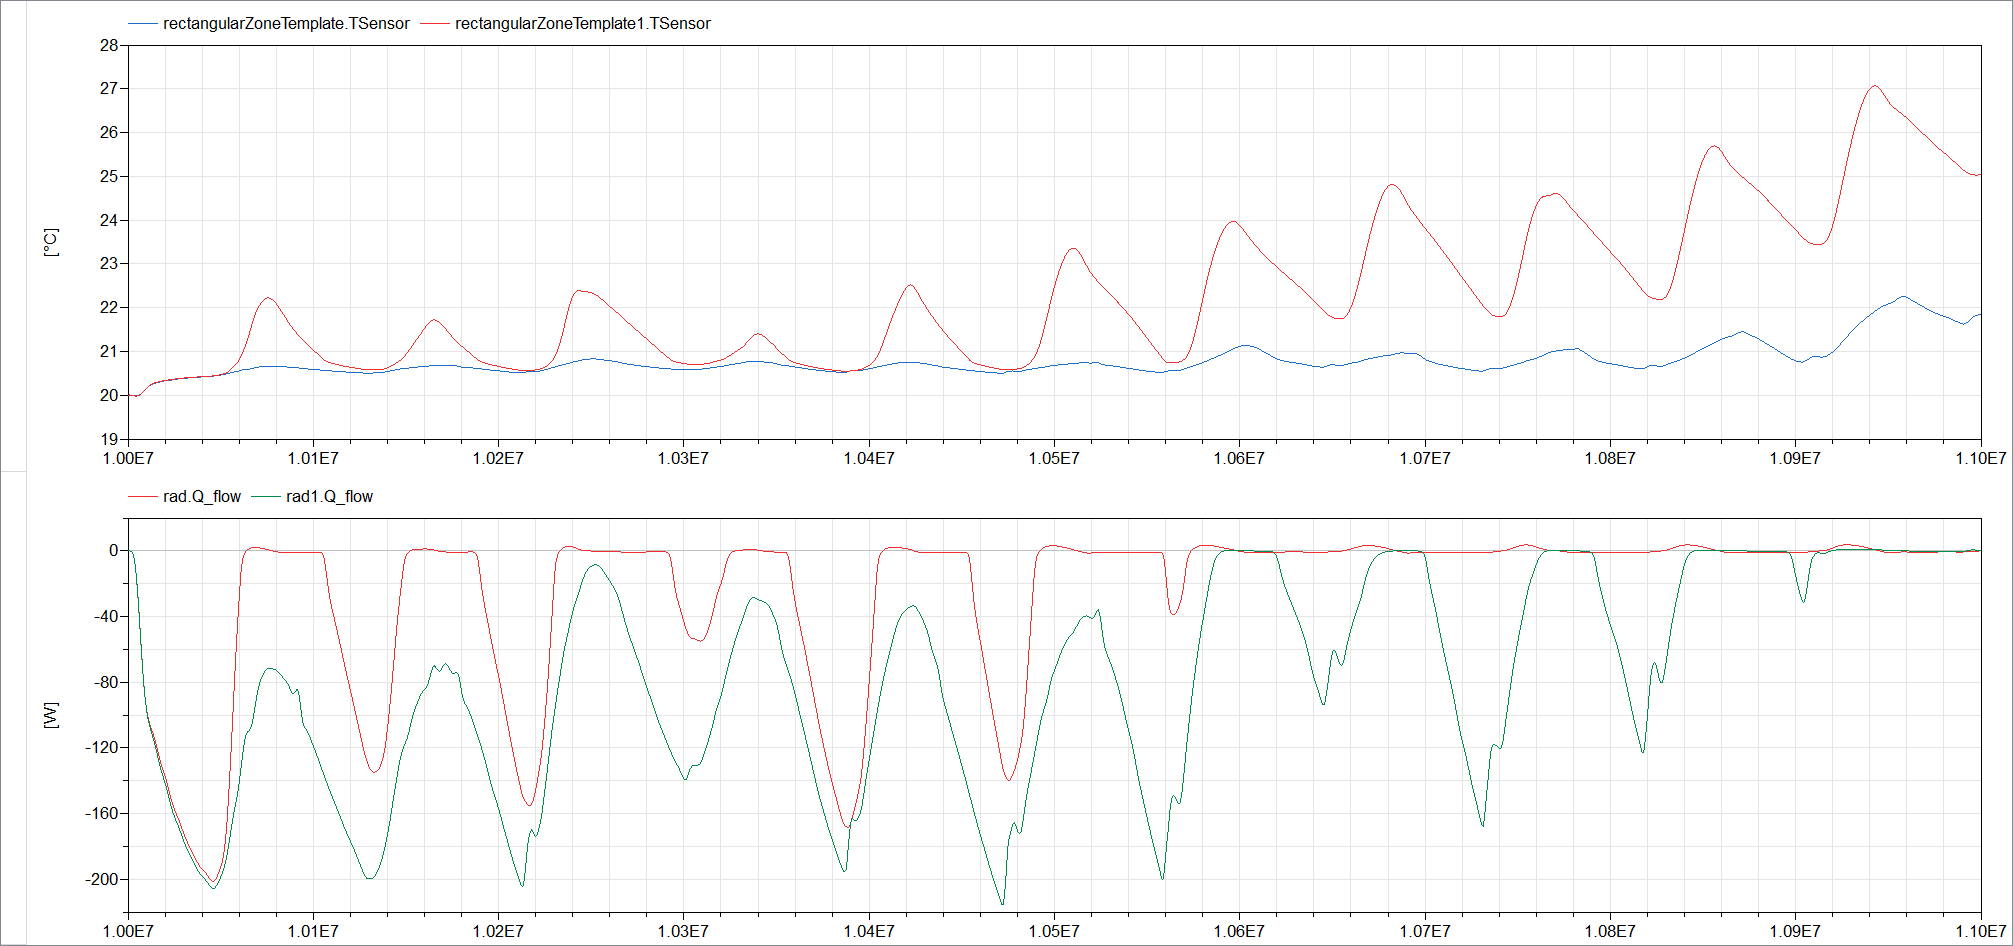
\includegraphics[scale=0.28]{Example6.png}
\caption{The model response for Example 6: zone temperatures and thermal power of radiators.}
\label{fig:res1}
\end{figure}
\begin{figure}[h]
	\centering
	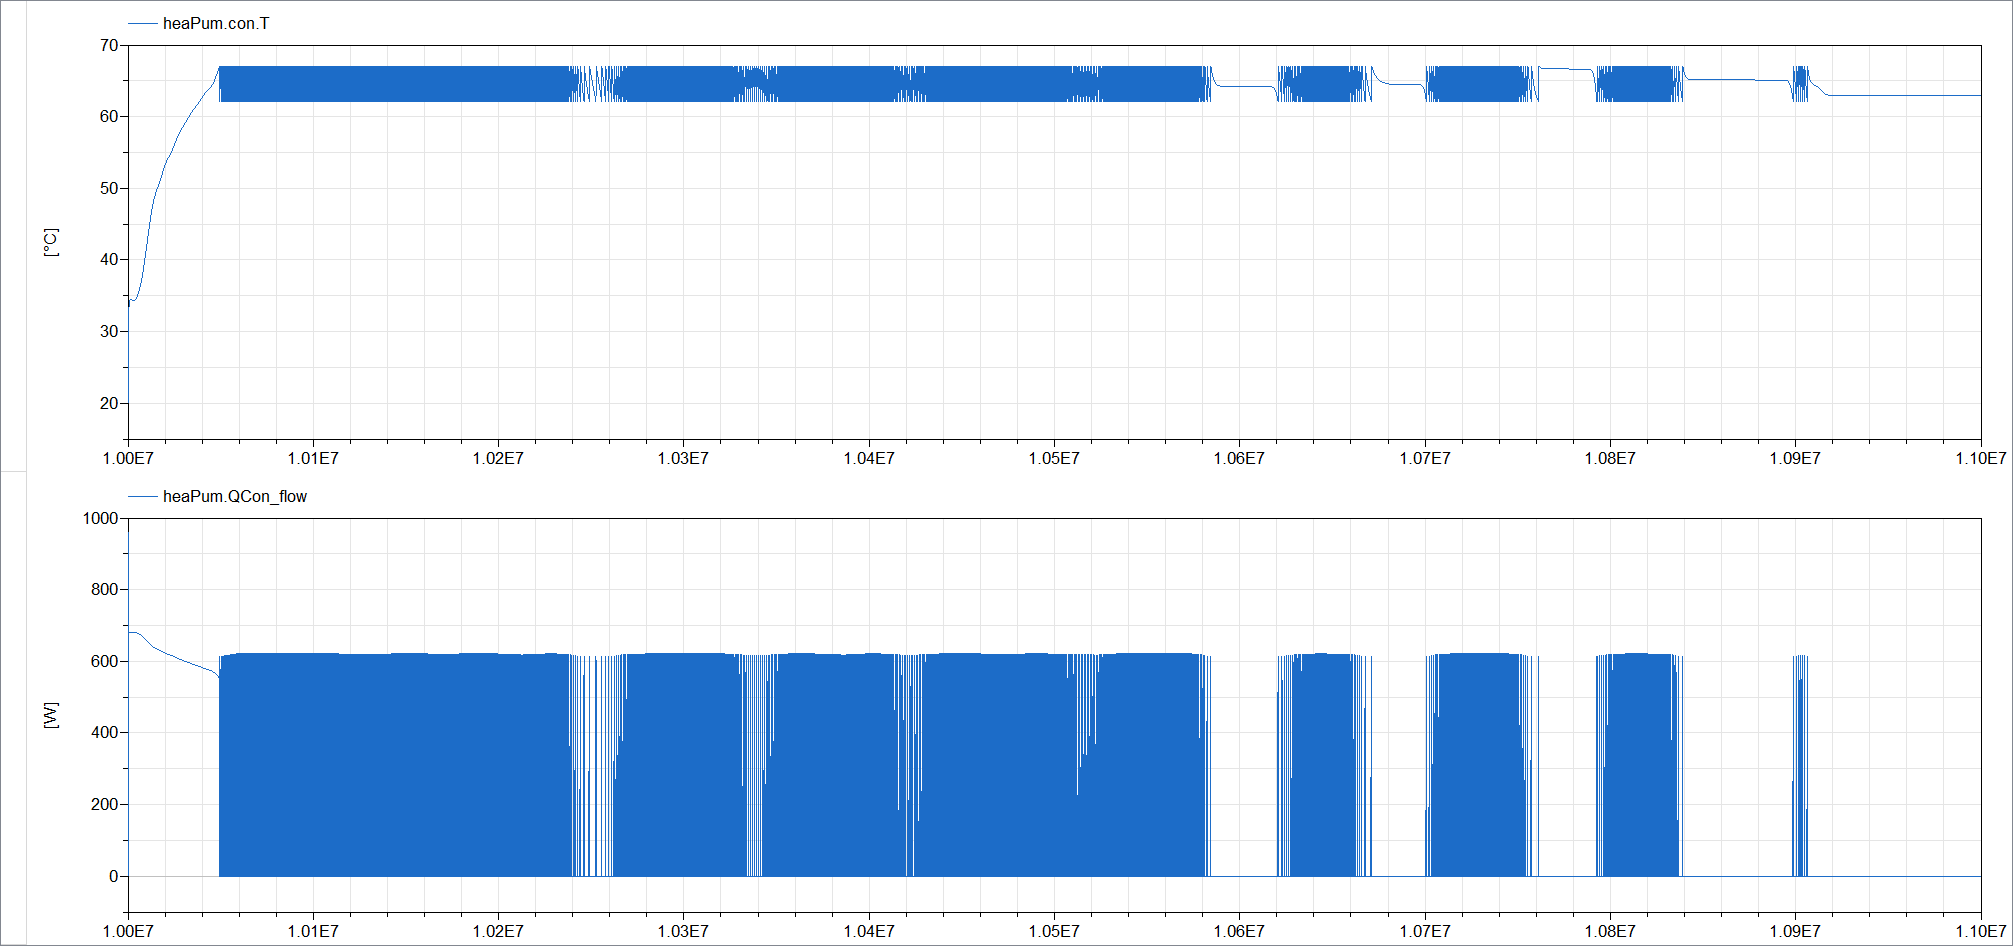
\includegraphics[scale=0.28]{Example6_bis.png}
	\caption{The model response for Example 6: heat pump condenser temperature and condensor thermal power.}
	\label{fig:res1_bis}
\end{figure}
\newpage

\section{Adding HVAC control}
\paragraph{Qualitative discussion}
This step adds a controller that disables the heat pump
when the supply water temperature exceeds 45$^{\circ}C$.


\paragraph{Required models}
This step requires the following components:
\begin{itemize}
\item \path{IDEAS.Fluid.Sensors.TemperatureTwoPort}
\item \path{Modelica.Blocks.Logical.Hysteresis}
\item \path{Modelica.Blocks.Math.BooleanToReal}
\end{itemize}

\paragraph{Instructions}
Before extending the previous step, add a temperature sensor between the storage tank
and the secondary circulation pump.
This measurement serves as an input to the hysteresis controller.
Now extend the model and configure the controller such that it switches to a \textit{false} signal below
40$^{\circ}C$ and to \textit{true} above 45$^{\circ}C$\footnote{Take into account that the measurement has units of Kelvin!}.\\

The output of the hysteresis controller is thus \textit{true} when the supply temperature is 
high enough and false otherwise.
This Boolean signal has to be converted in a real control signal that can be
accepted by the heat pump model.
For this purpose use the \path{BooleanToReal} block.
The heat pump already has a control signal. 
Since blocks cannot be removed from an extension of a model\footnote{Unless 
they are conditional, but we have not implemented that in this example.},
we can (in this case) work around the existing control signal
by changing the heat pump model input type to \path{enable_variable_speed=true}.
The model then accepts any real signal and connections to the other control 
signal are ignored. 


\paragraph{Side notes}
Note that the control signal of the heat pump could also have been used to disable
the circulation pumps.
However, disabling the circulation pump disables the flow of water,
which causes the temperature sensor output to remain fixed at
its last value.
Since this value, at the point of disabling the pump, was more then 45 degrees,
it would stay at that value and consequently the system would not be enabled again.
Note that this is not necessarily a model error, since the same problem could
occur in reality! This problem can be alleviated by modelling
heat losses in the sensor.\\


We have used a hysteresis controller to enable and disable the heat pump,
while we might as well have used a simple `greater or equal' comparison.
If there were no storage tank,
this would however introduce very rapid switching between turning the heat pump on
and off. Indeed, enabling the heat pump will, almost instantaneously increases the 
supply water temperature, causing the heat pump to be disabled again.
This effect is called chattering and can be very detrimental for the simulation speed 
and should therefore be avoided.
Note that this effect would also occur in practice if hysteresis controllers were not used.\\

In this example we use a trick to override the heat pump control signal, by enabling a new
control signal and by disabling the old one. This does not lead
to too many equations, since the Modelica specification states that 
connections to removed connectors or components should be ignored.


\paragraph{Reference result}
Figure~\ref{fig:res2} compares the results with the results without controller.
We see that indeed, the supply temperature is reduced significantly.
This causes the zone temperature to be slightly lower, up to about 0.25$^{\circ}C$.
The COP however increases from about 2.9 to about 3.1.
Consequently, the energy use over the period is reduced from 11.56~$kWh$
to 9.64~$kWh$. Note that this heating system configuration is still 
not efficient since the small flow rates still cause 
large temperatures to occur within the heat pump
and thus cause a small COP.
COP's of more than 5 are obtainable when using a bypass and a separate
pump to charge the storage tank.\\


To further play with this model, you can try to enable/disable the circulation pumps with the same control
signal and see what happens.
Secondly, you can set the heat pump control signal to 0.3 instead of 1,
which causes the heat pump to be modulated to 30\% thermal power.
This has a large impact on the COP since the temperature difference across the heat 
pump is reduced. 
However, the heat pump is unable to satisfy the heat demand.\\

\begin{figure}[h]
	\centering
	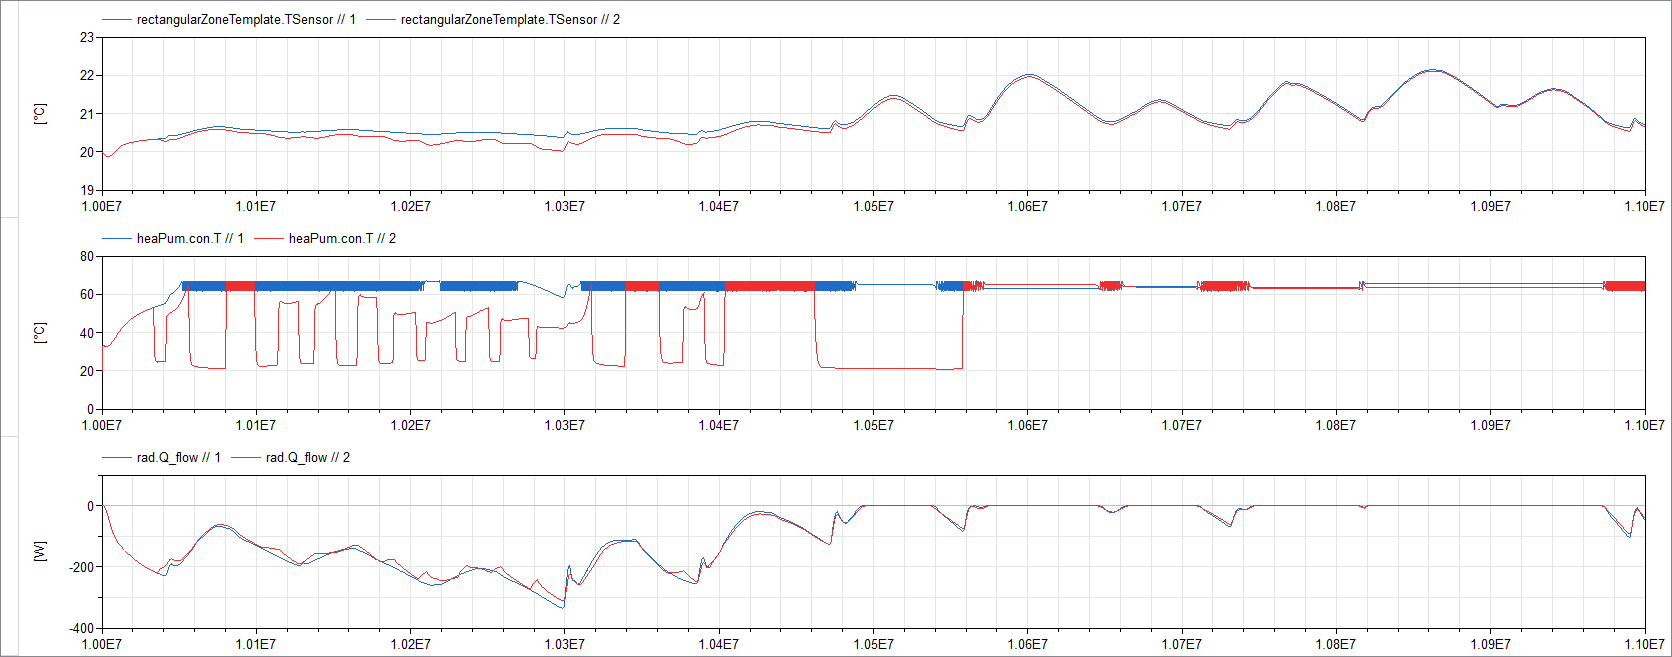
\includegraphics[width=\linewidth]{Example7.png}
	\caption{Comparison with (red) and without (blue) control for zone temperature, supply water temperature and radiator thermal power.}
	\label{fig:res2}
\end{figure}

\section{Workflow automation}
\paragraph{Qualitative discussion}
Extracting results from Modelica/Dymola can be tedious. 
Therefore several custom tools have been developed to facilitate exporting simulation results.
For time-series data, a generic CSV writer can be found in \path{IDEAS.Utilities.IO.Files.CSVWriter}.
This model generates a CSV file at a user-defined location that contains
data for each of the inputs of the block. 
The delimiter can be modified in the advanced parameter tab.
The model \path{IDEAS.Utilities.IO.Files.CombiTimeTableWriter}, does the same, albeit using a slightly
different file format which can be read directly back into Modelica using the
file reader \path{Modelica.Blocks.Sources.CombiTimeTable}.\\

In this example we will not output time series data, but instead a single value: the total
energy use at the end of the simulation, using the json file format. 
Note that the external library \path{ExternData} can be used to read json files.


\paragraph{Required models}
This step requires the following component:
\begin{itemize}
\item \path{IDEAS.Utilities.IO.Files.JSONWriter}
\end{itemize}

\paragraph{Instructions}
Add the model, choose a file path and indicate the appropriate time when 
the result should be saved.
Connect the appropriate signal to the input of the block.

\paragraph{Side notes}
Unless you specify a full path, the file will be generated in
the current working directory of your Dymola workspace.
See \path{File>Working directory>Browse} to inspect your current
working directory.
In this directory Dymola will generate all its own result files, C code, executables, etc.
It is good practice to set this directory where the resulting output does not cause a mess.
Note that by default Dymola sets this directory to the library directory when opening a library.

\paragraph{Reference result}
Check the contents of the generated file. 
Depending on the chosen value for the parameter \path{varKeys}, 
you should get something similar to:
\begin{verbatim}
{
  "Electrical energy [kWh]" : 1.2577137592e+01
}

\end{verbatim}


\section{Adding CO$_2$-controlled ventilation}
\paragraph{Qualitative discussion}
You will now add a CO$_2$-controlled ventilation system.
Add the occupancy model from Example 4 to one zone
and a fixed occupancy of 1 person to the other zone.
The ventilation system consists of two fans, two supply and two return air
VAVs (Variable Air Volume), a heat recovery unit and an outdoor air source.
The control consists of PI controllers with a set point of 1000 ppm.


\paragraph{Required models}
This step requires the following components:
\begin{itemize}
\item Custom occupant model from Example 4
\item \path{IDEAS.Fluid.Sources.OutsideAir}
\item \path{IDEAS.Fluid.Actuators.Dampers.PressureIndependent}
\item \path{IDEAS.Fluid.HeatExchangers.ConstantEffectiveness}
\item \path{IDEAS.Controls.Continuous.LimPID}
\item \path{Modelica.Blocks.Sources.Constant}
\end{itemize}


\paragraph{Important notes on Media}
\path{IDEAS.Media} contains a selection of medium \textit{packages}. 
Media packages contain the properties of media such as water or air.
Depending on the user requirements, the level of detail in these packages can change a lot.
For building applications, we use relatively simple media.
\begin{itemize}
	\item \path{IDEAS.Media.Water} assumes constant density and heat capacity and is thus
	a very simple medium.
	\item \path{IDEAS.Media.Antifreeze} contains media such as glycol water,
	which is a commonly used antifreeze.
	\item \path{IDEAS.Media.Air} is a simple air medium that 
	neglects the temperature dependency of the density of air to
	facilitate the numerics. By default, air is however compressible such that the density
	varies with pressure.
	\path{IDEAS.Media.Air} also contains water vapour,
	which allows the zone humidity to be computed. By default \path{IDEAS.Media.Air} does not model CO$_2$.
	However, any number of \textit{trace substances} can be added to the air model.
	This can be CO$_2$, VOC, dust, as long as it is simply transported together
	with the air stream without changing properties.
\end{itemize}


Note that you have to ensure that all coupled components must have the same Medium
for the model to work, i.e. if one zone is linked to a second zone through an air connection,
then each of them must have the same set of trace substances.

\paragraph{Instructions}
Extend this model from Example~7 and modify its existing medium declaration
to add CO$_2$, as follows:
\begin{verbatim}
extends Example7(
    redeclare package Medium = IDEAS.Media.Air(extraPropertiesNames={"CO2"}));
\end{verbatim}
For one zone, add the occupancy model from Example 4. 
You can copy it from \path{IDEAS.Examples.Tutorial.Example4}.
For the other zone, add a fixed occupancy of 1 person. For making a connection with the outside air we use \path{IDEAS.Fluid.Sources.OutsideAir},
which is similar to \path{IDEAS.Fluid.Sources.Boundary_pT} except that it 
automatically sets the outdoor dry bulb temperature and humidity. \\
%The outdoor CO$_2$ concentration is however not yet added automatically,
%causing it to be initialized to a default value of 0.
%We add the correct outdoor CO$_2$ concentration by
%enabling the input \path{C_in} using \path{use_C_in=true}.
%Connect the connector \path{weaBus} to the \path{SimInfoManager}
%and branch a bus off this connector as indicated in Figure~\ref{fig:bus}.
%Connect the connector \path{C_in} to the element \path{CEnv} of
%the newly created bus connector.\\

These were two tricky steps that can be quite complex for new users. 
Now add two supply and two return air VAVs
\footnote{A VAV works like an `air valve'. It has a built-in disc that is rotated to control the 
air flow rate. An internal controller rotates the disc such that a set point mass flow rate is tracked.
The set point equals \path{m_flow_nominal*y} where y is the control input.}.
Connect them to the \path{FluidPort}s of the zones. 
Ensure that the same port is not used twice, otherwise
the air will not enter the zone and simply return from one 
connection into the other at the port.
Also, use the convention that air enters in the blue port and leaves
through the white port.
For this exercise, assume that the VAV has a nominal flow rate of 100~$m^3/h$,
which equals 0.033~$kg/s$.
Assume a nominal pressure drop of 50~$Pa$ and
also add \path{dpFixed_nominal=50}, which causes the VAV
model to include a pressure drop of ducts, grills, filters or bends that are connected
at the inlet or outlet of the VAV. Next, add a supply fan and a return fan to which the VAVs
are connected in parallel. The fan pressure head is constant at 200~$Pa$
and its nominal flow rate is the sum of the VAV flow rates.
Finally, add a heat recovery heat exchanger with a constant effectiveness of 80 \%.
Choose reasonable nominal flow rates and set the nominal pressure drop to 100~$Pa$.
Make sure to use the new air Medium for all components that were just added.\\

The ventilation system model is now ready but cannot be simulated yet since
the control input of the VAVs is not set.
For this purpose, add two PI controllers and connect their outputs to the VAVs.
Connect the zone \path{ppm} outputs to the PI controller measurement inputs \path{u_m}.
Connect a constant set point of 1000~$ppm$ to the PI input \path{u_s}.
Add a minimum VAV opening of 10 \%.
Furthermore, set \path{k=0.005},  \path{Ti=300}, \path{reverseAction=false} and \path{controllerType=PI}. 
See the side notes for a motivation for these parameters, 
which is beyond the scope of this course. The schematic of the model you should have now is represented in Figure \ref{fig:ex9}.

%\begin{figure}
%\centering
%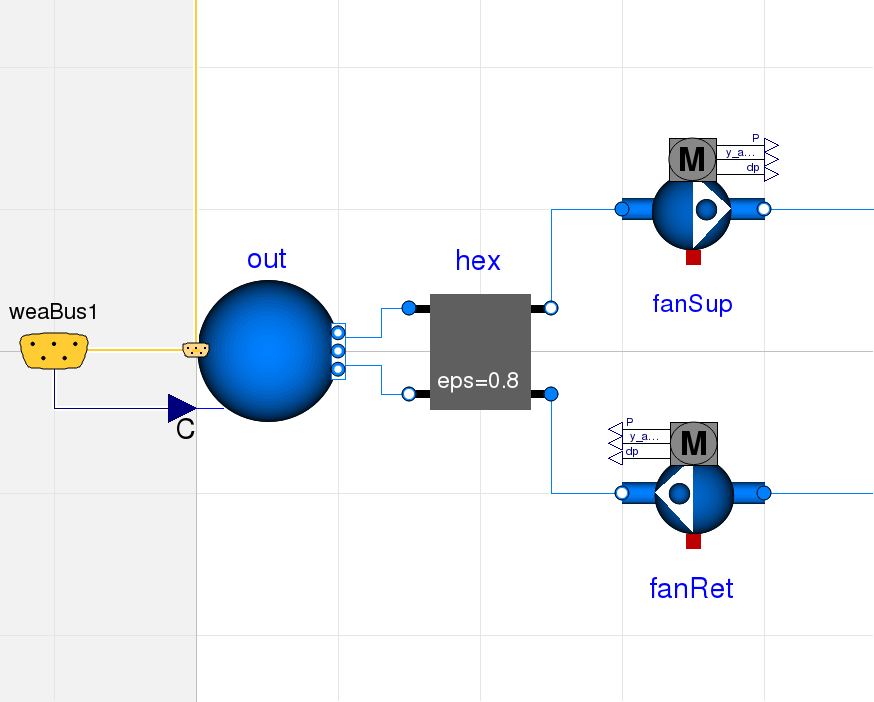
\includegraphics[scale=0.4]{Example9_bus.png}
%\caption{Example connection for outdoor air source and its inputs.}
%\label{fig:bus}
%\end{figure}

\begin{figure}[h]
	\centering
	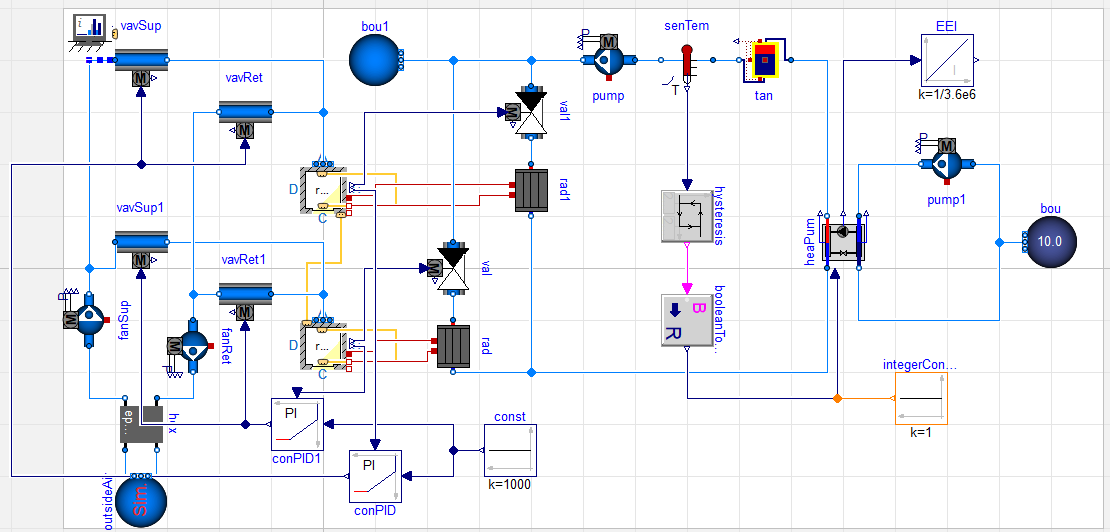
\includegraphics[width=\linewidth]{Schematic9.png}
	\caption{The schematic of Example 9.}
	\label{fig:ex9}
\end{figure}


\paragraph{Side notes}
Some background information on PI controllers, 
which are often used in buildings: 
PID controllers track a set point for some variable (in this case CO$_2$ concentration) \path{u_s} 
by checking the error compared to a measurement of that variable \path{u_m}
and by adjusting the control output \path{y}, which should be connected
to some actuator (in this case the VAV) that affects the measured variable.
The PID controller control internally computes the error $e=u_s-u_m$
and the output $y$ consists of three (optional) parts: 
\begin{enumerate}
\item the proportional part (P), which is proportional to $e$,
\item the integral part (I), which is proportional to the time integral $\int_0^\tau e \, \mathrm{d}t$
\item the differential part (D), which is proportional to the time derivative $\frac{ \mathrm{d} e}{ \mathrm{d} t}$.
\end{enumerate}
In a PI controller, the differential part is not included, etc.
A PID controller has an upper bound and lower bound for the output 
and further has three main parameters that should be tuned
for the system to work effectively.
Conceptually speaking, we have to tell the PID controller \textit{how much} it
should change its output for an observed error $e$.
To tune our PI, we used the following reasoning.
If the PI suddenly observes an error $e$ of 200~$ppm$,
we want the PI to change to fully open (assuming it was closed before).
The PI implementation is as follows 
\footnote{You can check \path{IDEAS.Controls.Continuous.LimPID} to verify this.}
\begin{equation}
y = ke + k/Ti\int e\mathrm{d}t.
\end{equation}
Since the integral term takes a while to respond,
an instantaneous step is only affected by $y=ke$.
Furthermore, we want $\Delta y = 1$  for $\Delta e = 200$,
which results in $k=0.005$.
The proportional term $k$ may not be sufficient
to track the set point. 
The remaining error can be compensated by the integral term, 
which can also be tuned using parameter $Ti$.
The reasoning here is as follows.
If an error of 200~$ppm$ persists for $Ti$ seconds,
we want the PI controller output to increase an additional 100 \% 
during that period.
In this case we chose $Ti=300$ seconds.
We have also set \path{reverseAction=false} to indicate to the PI,
that if the set point is larger than the measurement, the control output should
decrease instead of increase, which is the default. The same behaviour
can be obtained by  switch the two PI inputs.\\

Note that it may be tempting to set $k$ large and $Ti$ small
in order to get a controller that reacts very quickly. However,
if the system itself (the VAV and zone CO$_2$ concentration)
reacts with a delay, this can cause the system to oscillate.
You  can observe such behaviour when setting \path{riseTime=300} for the VAVs and
\path{Ti=60} in the PIs.
These oscillations cause the solver to take smaller time steps, 
which prolongs the simulation time.
Note that this is again not a software problem since these oscillations can/would occur 
in practice too!\\


By default, both the humidity of air, and the generation of water
vapor by occupants are simulated.
Furthermore, natural air infiltration in zones\footnote{See parameter n50.} is quite low, 
which can cause the zone humidity to increase strongly, 
even above 100 \% since water condensation
is not modelled by default.
This can explain seemingly wrong results when not modelling
a ventilation system.\\

Note that the default outdoor CO$_2$ concentration is fixed to 400~$ppm$.
It can be changed using the parameter \path{ppmCO2} in the 
\path{SimInfoManager}. You can even make it time-dependent
by overriding the value of the \path{RealExpression} block \path{CEnv}
in the \path{SimInfoManager}.

\paragraph{Reference result}
The zone temperature, CO$_2$ concentrations and 
PI control signals are plotted in Figure~\ref{fig:res4}.
Note the small overshoot of the PI controller outputs
and the exponential decay towards the outdoor CO$_2$
concentration when there are no occupants.


\begin{figure}[h]
\centering
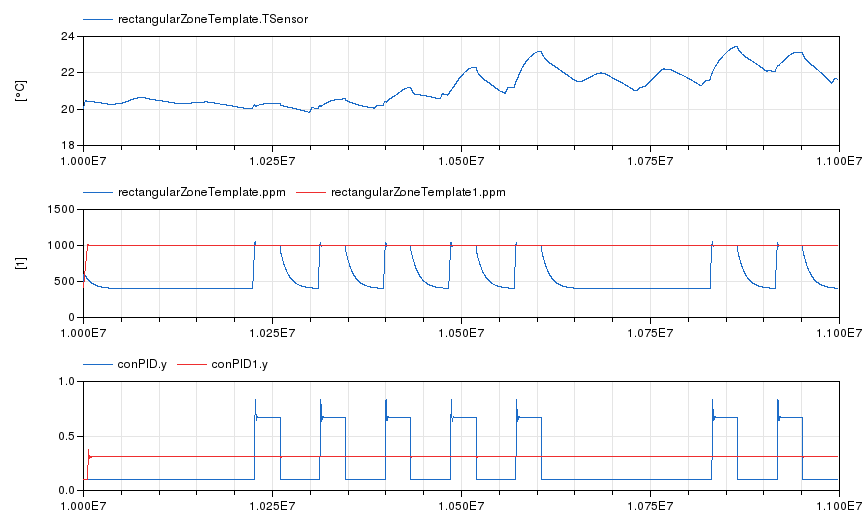
\includegraphics[width=\linewidth]{Example9.png}
\caption{Zone temperature, CO$_2$ concentrations and PI control signals.}
\label{fig:res4}
\end{figure}


\section{Computation time}
The models that you have just created are fairly slow
and computation time can easily explode when controller
oscillations occur or when the heat pump experiences frequent on/off switches. 
These effects cause a lot
of fast transients that force the solver to take small steps, 
which takes a lot of time.\\

Fortunately, there are many tricks that can be used to speed up the solver. 
The fundamental principle is that we remove small time constants from the problem,.
\path{IDEAS.Examples.Tutorial.Example10} implements changes that
cause the simulation to become 2 times faster.
If we do this systematically, and we remove \textbf{all} fast time constants,
we can use a different solver (Euler), 
using which the simulation time also becomes 2 times smaller
when using a fixed time step of 20 seconds.
These are modest improvements since this small example model behaves rather well.
However, for large models, the difference in computation time 
when using Euler integration can become a factor 1000.
The modifications however require a bit of knowledge about solvers 
and the models that you are using, including some of the more advanced parameters.
To learn more about this, we refer to \cite{Jorissen2015,Jorissen2018,phd}.

\begin{thebibliography}{9}
\bibitem{Jorissen2015} 
F. Jorissen, M. Wetter, and L. Helsen. Simulation Speed Analysis and Improvements of Modelica Models for Building Energy Simulation. In 11th International Modelica Conference, 59–69, Paris, 2015. doi: 10.3384/ ecp1511859

\bibitem{Jorissen2018}
F. Jorissen, M. Wetter, and L. Helsen. Simplifications for hydronic system models in modelica, Journal of Building Performance Simulation, 11:6, 639-654, 2018, doi: 10.1080/19401493.2017.1421263

\bibitem{phd}
F. Jorissen. \textit{Toolchain for Optimal Control and Design of Energy Systems in Buildings}. Phd thesis, Arenberg Doctoral School, KU Leuven, April 2018.

\end{thebibliography}


\end{document}